\documentclass[sigconf]{acmart}

% ---- remove ACM boilerplate: copyright box, reference block, conference header ----
\settopmatter{printacmref=false, printccs=false, printfolios=true}
\setcopyright{none}
\renewcommand\footnotetextcopyrightpermission[1]{}
\acmDOI{}
\acmISBN{}
\acmConference{}{}{}

\usepackage{amsmath}
\usepackage{booktabs}
\usepackage{algorithm}
\usepackage[noend]{algpseudocode}
\usepackage{tikz}
\usetikzlibrary{arrows.meta, positioning, fit, calc, backgrounds}

\algrenewcommand\algorithmicrequire{\textbf{Input:}}
\algrenewcommand\algorithmicensure{\textbf{Output:}}
\algrenewcommand\alglinenumber[1]{\scriptsize #1:}
\newcommand{\Perm}{\operatorname{Perm}}
\newcommand{\topm}{\operatorname{top}}
\newcommand{\core}{\textsc{CoRE}}
\setlength{\emergencystretch}{1.5em}

\begin{document}

\title{Which Condition Fits? Multi-Label Diagnosis with Supporting Evidence from Symptom Description}

\author{Niyaaz Baines}
\affiliation{\institution{University of Victoria}}
\email{nbaines@uvic.ca}
\author{Eduardo Kallina de Paula}
\affiliation{\institution{University of Victoria}}
\email{ekallinadepaula@uvic.ca}
\author{Thiago Vasconcelos Pinheiro Lopes}
\affiliation{\institution{University of Victoria}}
\email{thiagovplopes@uvic.ca}
\author{Priyanshkumar Ghanshyambhai Patel}
\affiliation{\institution{University of Victoria}}
\email{priyanshkumarghansh1@uvic.ca}

\renewcommand{\shortauthors}{Baines, Kallina de Paula, Lopes, and Patel}

\begin{abstract}
ADHD, anxiety, and depression share symptoms such as inattention, restlessness, and irritability, yet most text classifiers assign one condition per description. We propose \core{} (Co-occurring condition classification with Rationale Extraction), which returns the best-fitting condition for a self-reported symptom description, any other consistent conditions, and the phrases that support each. \core{} learns from Reddit posts with weak multi-label targets drawn from the source community and from self-reported diagnoses, masks condition names, models co-occurrence with an order-averaged classifier chain, and selects evidence by phrase occlusion. The seeded implementation reproduces its results from one quickstart script. Code: \href{https://github.com/eduardokdp/Which-Condition-Fits-}{github.com/eduardokdp/\allowbreak Which-Condition-Fits-}.
\end{abstract}

\keywords{Mental health, multi-label classification, classifier chains, rationale extraction}

\maketitle
\pagestyle{plain}

\section{Introduction}
Most text-based methods reviewed in Milestone 2 separate one condition from healthy controls or assign one label per post. Multi-label work such as SMHD \cite{cohan2018smhd} and the comorbidity ensemble of Souza et al. \cite{souza2021deep} gives no evidence for its predictions, and rationale methods \cite{lei2016rationalizing, deyoung2020eraser} have not been applied to co-occurring conditions. \core{} combines existing techniques into a new pipeline with three parts: (i) weak multi-label supervision from self-reported diagnoses, with condition names masked; (ii) an order-averaged classifier chain in which the score of one condition depends on the others; and (iii) per-condition occlusion rationales that expose phrases shared by several conditions.

\begin{figure*}[t]
\centering
\resizebox{\textwidth}{!}{%
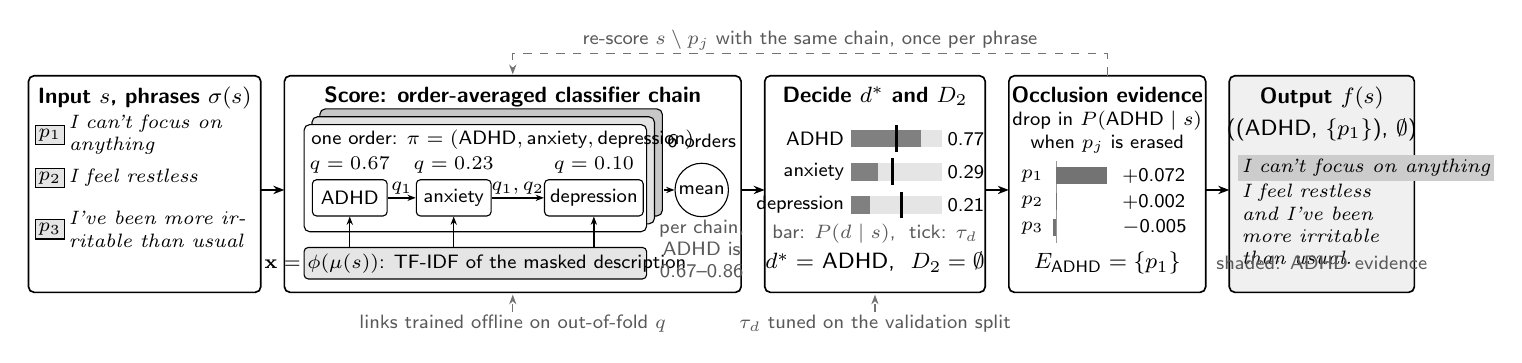
\begin{tikzpicture}[x=1cm, y=1cm, font=\footnotesize\sffamily,
  stage/.style={draw, rounded corners=2pt, line width=0.6pt},
  ttl/.style={font=\footnotesize\sffamily\bfseries, anchor=north, inner sep=1pt},
  small/.style={font=\scriptsize\sffamily, inner sep=1pt},
  note/.style={font=\scriptsize\sffamily, text=black!65, inner sep=1pt},
  arr/.style={-{Stealth[length=4pt]}, line width=0.8pt},
  thin/.style={-{Stealth[length=3pt]}, line width=0.5pt},
  link/.style={draw, rounded corners=1.5pt, fill=white, minimum height=0.46cm, inner sep=2pt, font=\scriptsize\sffamily},
  darr/.style={-{Stealth[length=3.5pt]}, dashed, black!55}]
\def\H{2.75}
% stage frames: x-origin / width
\foreach \x/\w in {0/2.95, 3.25/5.8, 9.35/2.8, 12.45/2.5}{\draw[stage] (\x,0) rectangle ++(\w,-\H);}
\draw[stage, fill=black!6] (15.25,0) rectangle ++(2.35,-\H);
\foreach \a/\b in {2.95/3.25, 9.05/9.35, 12.15/12.45, 14.95/15.25}{\draw[arr] (\a,-1.45) -- (\b,-1.45);}

% ---------- 1. input and phrases (x = 0, width 2.95) ----------
\begin{scope}[xshift=0cm]
\node[ttl] at (1.475,-0.1) {Input $s$, phrases $\sigma(s)$};
\foreach \j/\y/\txt in {1/-0.75/{I can't focus on anything}, 2/-1.3/{I feel restless}, 3/-1.95/{I've been more irritable than usual}}{
  \node[draw, fill=black!10, inner sep=1.3pt, font=\scriptsize] at (0.27,\y) {$p_{\j}$};
  \node[anchor=west, text width=2.35cm, align=left, inner sep=1pt, font=\scriptsize\itshape] at (0.47,\y) {\txt};}
\end{scope}

% ---------- 2. order-averaged classifier chain (x = 3.25, width 5.8) ----------
\begin{scope}[xshift=3.25cm]
\node[ttl] at (2.9,-0.1) {Score: order-averaged classifier chain};
\foreach \o/\g in {0.2/22, 0.1/11}{\draw[rounded corners=2pt, fill=black!\g] (0.25+\o,-0.62+\o) rectangle (4.6+\o,-1.98+\o);}
\draw[rounded corners=2pt, fill=white] (0.25,-0.62) rectangle (4.6,-1.98);
\node[small, anchor=north west] at (0.3,-0.64) {one order: $\pi=(\text{ADHD},\text{anxiety},\text{depression})$};
\node[link, minimum width=0.95cm] (L1) at (0.83,-1.55) {ADHD};
\node[link, minimum width=0.95cm] (L2) at (2.15,-1.55) {anxiety};
\node[link, minimum width=1.1cm]  (L3) at (3.93,-1.55) {depression};
\draw[thin] (L1) -- node[above, small] {$q_1$} (L2);
\draw[thin] (L2) -- node[above, small] {$q_1,q_2$} (L3);
\foreach \L/\q in {L1/0.67, L2/0.23, L3/0.10}{\node[small, anchor=south] at ([yshift=1pt]\L.north) {$q=\q$};}
\draw[fill=black!10, rounded corners=1.5pt] (0.25,-2.18) rectangle (4.6,-2.58);
\node[small] at (2.425,-2.38) {$\mathbf{x}=\phi(\mu(s))$: TF-IDF of the masked description};
\foreach \L in {L1,L2,L3}{\draw[thin] (\L |- 0,-2.18) -- (\L.south);}
\node[small] at (5.3,-0.82) {6 orders};
\node[draw, circle, fill=white, inner sep=1pt, small] (avg) at (5.3,-1.45) {mean};
\draw[thin] (4.82,-1.45) -- (avg.west);
\node[note, align=center] at (5.3,-2.2) {per chain,\\ ADHD is\\ 0.67--0.86};
\end{scope}

% ---------- 3. decide (x = 9.35, width 2.8) ----------
\begin{scope}[xshift=9.35cm]
\node[ttl] at (1.4,-0.1) {Decide $d^{*}$ and $D_2$};
\foreach \lab/\v/\t/\y in {ADHD/0.77/0.50/-0.8, anxiety/0.29/0.45/-1.22, depression/0.21/0.55/-1.64}{
  \node[small, anchor=east] at (1.05,\y) {\lab};
  \fill[black!10] (1.1,\y-0.11) rectangle (2.25,\y+0.11);
  \fill[black!50] (1.1,\y-0.11) rectangle ({1.1+1.15*\v},\y+0.11);
  \draw[line width=1.1pt] ({1.1+1.15*\t},\y-0.17) -- ({1.1+1.15*\t},\y+0.17);
  \node[small, anchor=west] at (2.28,\y) {\v};}
\node[note] at (1.4,-2.0) {bar: $P(d\mid s)$, \ tick: $\tau_d$};
\node[anchor=north, inner sep=1pt] at (1.4,-2.2) {$d^{*}=$ ADHD, \ $D_2=\emptyset$};
\end{scope}

% ---------- 4. occlusion evidence (x = 12.45, width 2.5) ----------
\begin{scope}[xshift=12.45cm]
\node[ttl] at (1.25,-0.1) {Occlusion evidence};
\node[small, align=center] at (1.25,-0.72) {drop in $P(\text{ADHD}\mid s)$\\ when $p_j$ is erased};
\draw[black!40] (0.6,-1.08) -- (0.6,-2.12);
\foreach \j/\v/\txt/\y in {1/0.072/{+0.072}/-1.27, 2/0.002/{+0.002}/-1.6, 3/-0.005/{$-$0.005}/-1.93}{
  \node[small] at (0.3,\y) {$p_{\j}$};
  \fill[black!55] (0.6,\y-0.11) rectangle ({0.6+9*\v},\y+0.11);
  \node[small, anchor=west] at (1.4,\y) {\txt};}
\node[anchor=north, inner sep=1pt] at (1.25,-2.2) {$E_{\text{ADHD}}=\{p_1\}$};
\end{scope}

% ---------- 5. output (x = 15.25, width 2.35) ----------
\begin{scope}[xshift=15.25cm]
\node[ttl] at (1.175,-0.1) {Output $f(s)$};
\node[anchor=north, inner sep=1pt] at (1.175,-0.5) {((ADHD, $\{p_1\}$), $\emptyset$)};
\node[anchor=north west, inner sep=1.5pt, fill=black!20, font=\scriptsize\itshape] at (0.1,-1.0) {I can't focus on anything};
\node[anchor=north west, text width=2.15cm, align=left, inner sep=1.5pt, font=\scriptsize\itshape] at (0.1,-1.32) {I feel restless and I've been more irritable than usual.};
\node[note, anchor=north] at (1.175,-2.25) {shaded: ADHD evidence};
\end{scope}

% ---------- occlusion re-scoring loop (stage 4 -> stage 2) ----------
\draw[darr] (13.7,0) -- (13.7,0.28) -- node[above, note] {re-score $s\setminus p_j$ with the same chain, once per phrase} (6.15,0.28) -- (6.15,0.02);
% ---------- where training enters ----------
\draw[darr] (6.15,-3.0) -- (6.15,-\H-0.03);
\node[note, anchor=north] at (6.15,-3.0) {links trained offline on out-of-fold $q$};
\draw[darr] (10.75,-3.0) -- (10.75,-\H-0.03);
\node[note, anchor=north] at (10.75,-3.0) {$\tau_d$ tuned on the validation split};
\end{tikzpicture}}
\caption{\core{} on the running example, with the quickstart model's values. The chain box unrolls one of the six label orders; occlusion re-scores the description once per erased phrase, for every predicted condition.}
\label{fig:pipeline}
\end{figure*}

\section{Problem Definition: Input and Output}
Let $D=\{d_1,\dots,d_k\}$ be an ordered set of conditions ($k=3$: ADHD, anxiety, depression) and $S$ a set of self-reported descriptions. A segmentation function $\sigma$ splits $s\in S$ at sentence ends and at clause boundaries where a comma or conjunction precedes a subject such as ``I'' or ``my'', giving phrases $\sigma(s)=\langle p_1,\dots,p_n\rangle$, $n\ge1$; $s\setminus p_j$ is $s$ with $p_j$ erased. Refining Milestone 1, \core{} computes
\begin{equation}
f(s)=\big((d^{*},E^{*}),\ \{(d_i,E_i)\}_{i=1}^{m}\big),\quad 0\le m\le k-1,
\end{equation}
where $d^{*}\in D$ is the primary condition, $d_1,\dots,d_m\in D\setminus\{d^{*}\}$ are distinct secondary conditions, and $E^{*},E_i\subseteq\sigma(s)$ are their evidence sets. The secondary set may be empty, and a phrase may belong to several evidence sets, because a symptom such as restlessness can support more than one condition. Figure~\ref{fig:pipeline} follows the running example of Milestone 1, whose description splits into the phrases $p_1$, $p_2$, and $p_3$, from input to output; Algorithm~\ref{alg:core} gives the pseudo-code.

\section{Proposed Method}
\textbf{Weak multi-label supervision.} A training post $s$ comes from a community $c(s)$ (r/ADHD, r/Anxiety, r/depression); $c_d$ is the community of $d$. Its target is
\begin{equation}
y_d(s)=\mathbf{1}[c(s)=c_d]\ \lor\ \mathbf{1}[d\in R(s)],
\end{equation}
where $R(s)$ holds the conditions named in first-person diagnosis statements (``I was diagnosed with'', ``I also have'', ``my\dots''), rejecting negated, hedged (``I wonder if I have''), and third-party (``my brother has'') ones. Community labels alone are single-label, whereas self-reports are precise and are how CLPsych and SMHD label users \cite{coppersmith2015clpsych, cohan2018smhd}. A mask $\mu$ then replaces condition names, but not symptom words such as ``anxious'', with one token, so the model must rely on symptom language.

\textbf{Representation.} The vector $\mathbf{x}=\phi(\mu(s))$ is a sublinear TF-IDF vector over word uni- and bigrams $t$ formed between masked names, so the mask is never a feature:
\begin{equation}
x_t=\frac{(1+\ln\mathrm{tf}_{t})\,\mathrm{idf}_t}{Z},\qquad \mathrm{idf}_t=\ln\frac{1+N}{1+\mathrm{df}_t}+1,
\end{equation}
with $\mathrm{tf}_t\ge1$ the count of $t$ in $\mu(s)$ ($x_t=0$ if $t$ is absent), $\mathrm{df}_t$ the number of the $N$ training posts containing $t$, and $Z$ the $\ell_2$ norm. It keeps the pronoun ``I'' and contractions such as ``can't'', since first-person pronouns mark depression \cite{rude2004language}. A linear representation is cheap to recompute, which occlusion needs.

\textbf{Order-averaged classifier chain.} Binary relevance scores each condition alone and ignores co-occurrence; a classifier chain \cite{read2011classifier} conditions each label on the previous ones but depends on an arbitrary order. For every order $\pi\in\Perm(D)$, link $j$ computes
\begin{equation}
q^{\pi}_{\pi_j}=\mathrm{sig}\big(\mathbf{w}_{\pi,j}^{\top}[\mathbf{x};\,q^{\pi}_{\pi_1},\dots,q^{\pi}_{\pi_{j-1}}]+b_{\pi,j}\big),
\end{equation}
and $P(d\mid s)=\frac{1}{k!}\sum_{\pi}q^{\pi}_{d}$ averages the $3!=6$ chains. The order matters: for the running example, a single chain's ADHD score ranges from 0.67 to 0.86 across orders (Figure~\ref{fig:pipeline}), and the mean removes this dependence. Each link is an $\ell_2$-regularised, class-weighted logistic regression ($C=1$). In training, the predecessor inputs are 5-fold out-of-fold probabilities, so each link sees the same kind of input as at inference.

\textbf{Decision rule.} The proposal requires a primary condition for every description, so $d^{*}=\arg\max_{d}P(d\mid s)$, and $D_2=\{d\ne d^{*}:P(d\mid s)\ge\tau_d\}$ are the secondary conditions. Each threshold $\tau_d$ is the value on a 0.05-step grid that maximises the F1 of $d$ on the validation split, which corrects for different base rates.

\textbf{Occlusion rationales.} The contribution of $p_j$ to $d$ is $\Delta_d(p_j)=P(d\mid s)-P(d\mid s\setminus p_j)$, and $E_d$ keeps the top $\lceil n/2\rceil$ phrases with $\Delta_d(p_j)>\delta=0.01$. Erasure \cite{li2016erasure} needs no rationale labels, works with any scorer, and targets ERASER comprehensiveness \cite{deyoung2020eraser}. A phrase in two evidence sets is reported as a shared symptom.

\begin{algorithm}[t]
\caption{\core{} training and inference}\label{alg:core}
\small
\begin{algorithmic}[1]
\Require posts $\mathcal{S}$ with communities; conditions $D$; description $s$
\Ensure $f(s)=((d^{*},E_{d^{*}}),\{(d,E_d):d\in D_2\})$
\For{$t\in\mathcal{S}$} $\mathbf{y}(t)\gets$ Eq.~(2);\ $t\gets\mu(t)$ \EndFor
\State split $\mathcal{S}$ 70/15/15 (stratified, seed 42);\ $X\gets\phi(\mathcal{S}_{tr})$
\For{$\pi\in\Perm(D)$} $Q\gets\mathbf{0}$
  \For{$j=1$ \textbf{to} $k$} $X_j\gets[X;\,Q_{\pi_1..\pi_{j-1}}]$
    \State $Q_{\pi_j}\gets$ \Call{OutOfFold}{$X_j,\mathbf{y}_{\pi_j}$};\ $h_{\pi,j}\gets$ \Call{LogReg}{$X_j,\mathbf{y}_{\pi_j}$}
  \EndFor
\EndFor
\State $\tau_d\gets\arg\max_{\tau}\mathrm{F1}_d(\tau)$ on $\mathcal{S}_{va}$, for each $d\in D$
\State $\langle p_1,\dots,p_n\rangle\gets\sigma(s)$;\ $\mathbf{P}\gets$ \Call{Score}{$s$}
\State $d^{*}\gets\arg\max_d P_d$;\ $D_2\gets\{d\ne d^{*}:P_d\ge\tau_d\}$
\For{$d\in\{d^{*}\}\cup D_2$}
  \State $\Delta_d(p_j)\gets P_d-\textproc{Score}(s\setminus p_j)_d$ for $j=1,\dots,n$
  \State $E_d\gets\topm_{\lceil n/2\rceil}\{p_j:\Delta_d(p_j)>\delta\}$
\EndFor
\Statex \textsc{Score}$(t)$: mean over $\pi$ of the chain outputs (Eq.~4) on $\phi(\mu(t))$
\end{algorithmic}
\end{algorithm}



\section{Implementation}
The repository follows the FAIR principles \cite{wilkinson2016fair} and the course template: a driver, \texttt{src/main.py}, calls \texttt{dataprep} (Eq.~2, masking, splits), \texttt{core} (one module per stage of Section~3), and \texttt{eval} (metrics and baselines), which share \texttt{cmn} (configuration, seeding, I/O). The full run uses the 2019 r/ADHD, r/Anxiety, and r/depression files of the public-domain Reddit Mental Health Dataset \cite{low2020reddit}, with up to 5,000 posts per community after removing deleted posts, bots, duplicates, and all but one post per author, which prevents author leakage across splits.

\textbf{Quickstart and reproducibility.} \texttt{quickstart.sh} installs the pinned requirements, runs 18 unit and reproducibility tests, and runs the pipeline in about a minute on 1,786 public Reddit posts bundled with the code (350 per community used). Because r/ADHD and the other two communities come from different public collections, these scores are indicative only. Seeding (42) and a SHA-256 check of the predictions make runs repeatable. On 158 test posts, \core{} reaches a micro-F1 of 0.65 (95\% bootstrap CI 0.60--0.70), within noise of both baselines, so whether the chain's extra cost (18 logistic regressions instead of 3) pays off is left to Milestone 4; deleting its evidence lowers the predicted probability by 0.12, against 0.02 for as many random phrases. For the running example it returns ADHD with evidence $p_1$ (Figure~\ref{fig:pipeline}), the primary condition of the Milestone 1 target.

\vspace{1mm}\noindent\textbf{Contributions.} Niyaaz: formal definition, abstract, introduction; Eduardo: method, references; Thiago: pseudo-code, implementation; Priyansh: Figure~1, integration. \textbf{Use of AI} (Level D): parts of the code and text were drafted with Claude (Anthropic), then reviewed, run, and revised by the authors.

\begin{thebibliography}{10}
\bibitem{cohan2018smhd} Arman Cohan, Bart Desmet, Andrew Yates, et al. 2018. SMHD: A Large-Scale Resource for Exploring Online Language Usage for Multiple Mental Health Conditions. In \textit{Proc. COLING}. 1485--1497.
\bibitem{coppersmith2015clpsych} Glen Coppersmith, Mark Dredze, Craig Harman, et al. 2015. CLPsych 2015 Shared Task: Depression and PTSD on Twitter. In \textit{Proc. CLPsych Workshop}. 31--39.
\bibitem{deyoung2020eraser} Jay DeYoung, Sarthak Jain, Nazneen Fatema Rajani, et al. 2020. ERASER: A Benchmark to Evaluate Rationalized NLP Models. In \textit{Proc. ACL}. 4443--4458.
\bibitem{lei2016rationalizing} Tao Lei, Regina Barzilay, and Tommi Jaakkola. 2016. Rationalizing Neural Predictions. In \textit{Proc. EMNLP}. 107--117.
\bibitem{li2016erasure} Jiwei Li, Will Monroe, and Dan Jurafsky. 2016. Understanding Neural Networks through Representation Erasure. arXiv:1612.08220.
\bibitem{low2020reddit} Daniel M. Low, Laurie Rumker, Tanya Talkar, et al. 2020. Natural Language Processing Reveals Vulnerable Mental Health Support Groups and Heightened Health Anxiety on Reddit during COVID-19. \textit{J. Medical Internet Research} 22, 10 (2020), e22635.
\bibitem{read2011classifier} Jesse Read, Bernhard Pfahringer, Geoff Holmes, and Eibe Frank. 2011. Classifier Chains for Multi-label Classification. \textit{Machine Learning} 85, 3 (2011), 333--359.
\bibitem{rude2004language} Stephanie Rude, Eva-Maria Gortner, and James Pennebaker. 2004. Language Use of Depressed and Depression-Vulnerable College Students. \textit{Cognition and Emotion} 18, 8 (2004), 1121--1133.
\bibitem{souza2021deep} Vanessa Souza, J\'eferson Nobre, and Karin Becker. 2021. A Deep Learning Ensemble to Classify Anxiety, Depression, and their Comorbidity from Texts of Social Networks. \textit{J. Information and Data Management} 12, 3 (2021).
\bibitem{wilkinson2016fair} Mark D. Wilkinson, Michel Dumontier, IJsbrand Jan Aalbersberg, et al. 2016. The FAIR Guiding Principles for Scientific Data Management and Stewardship. \textit{Scientific Data} 3 (2016), 160018.
\end{thebibliography}

\end{document}
